% Determinant : developpement par rapport a la colonne 1
% Compilation : latex + dvisvgm --no-fonts (pipeline Makefile du book)
\documentclass{standalone}
\usepackage{amsmath}
\usepackage{tikz}
\usetikzlibrary{matrix, positioning, calc, backgrounds}

\begin{document}
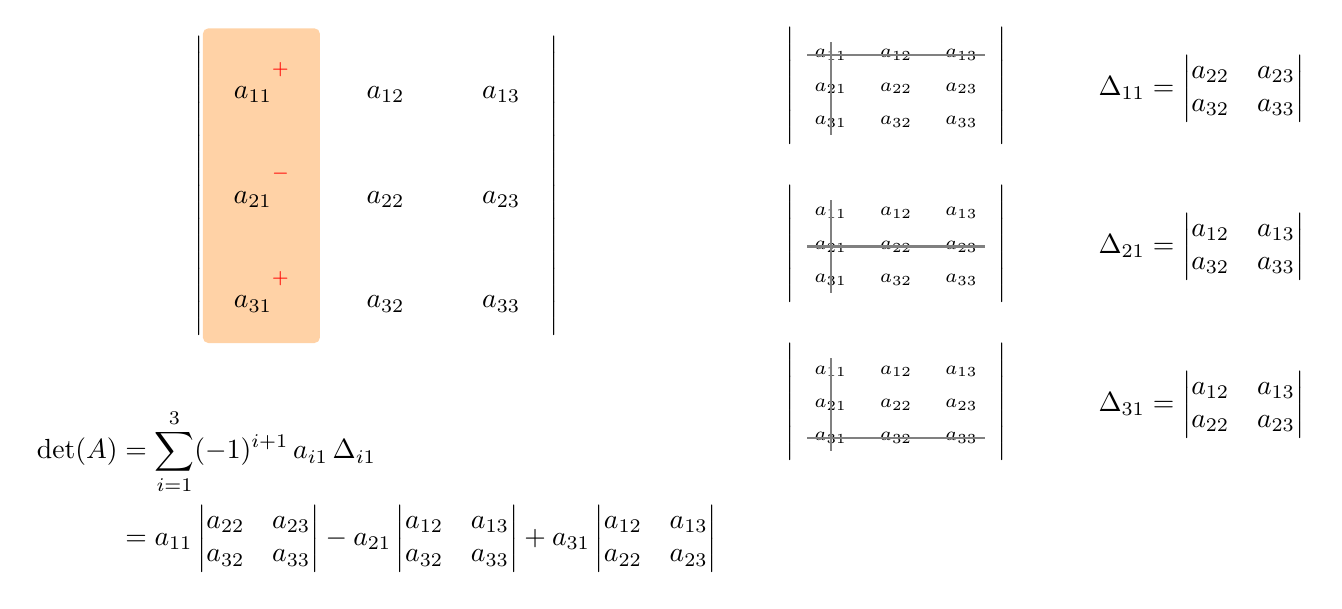
\begin{tikzpicture}[
  petit/.style={matrix of math nodes,
                nodes={inner sep=2.5pt, font=\scriptsize},
                row sep=3pt, column sep=7pt,
                left delimiter=|, right delimiter=|}
]

  %=========================================================
  % 1. Matrice A, colonne 1 mise en evidence
  %=========================================================
  \matrix (A) [petit,
               nodes={inner sep=6pt, font=\normalsize},
               row sep=1em, column sep=1.6em]
  {
    a_{11}\overset{\textcolor{red}{+}}{\phantom{b}} & a_{12} & a_{13} \\
    a_{21}\overset{\textcolor{red}{-}}{\phantom{b}} & a_{22} & a_{23} \\
    a_{31}\overset{\textcolor{red}{+}}{\phantom{b}} & a_{32} & a_{33} \\
  };

  \begin{scope}[on background layer]
    \fill[orange!35, rounded corners=2pt]
      ($(A-1-1.north west)+(-5pt,5pt)$) rectangle
      ($(A-3-1.south east)+(5pt,-5pt)$);
  \end{scope}

  %=========================================================
  % 2. Formule de developpement (signes = alignes,
  %    det(A) non repete)
  %=========================================================
  \node[below=2.2em of A.south] (eq)
    {$\begin{aligned}
       \det(A)&=\sum_{i=1}^{3}(-1)^{i+1}\,a_{i1}\,\Delta_{i1}\\
              &=a_{11}\begin{vmatrix} a_{22}&a_{23}\\ a_{32}&a_{33}\end{vmatrix}
               -a_{21}\begin{vmatrix} a_{12}&a_{13}\\ a_{32}&a_{33}\end{vmatrix}
               +a_{31}\begin{vmatrix} a_{12}&a_{13}\\ a_{22}&a_{23}\end{vmatrix}
     \end{aligned}$};

  %=========================================================
  % 3. Construction des mineurs : on barre la ligne i et la
  %    colonne 1. Colonne alignee verticalement avec (A, eq)
  %=========================================================

  % --- Mineur Delta_11 : on barre la ligne 1 ---
  \matrix (M1) [petit, anchor=north west] at ([xshift=7.5cm]A.north west)
  {
    a_{11} & a_{12} & a_{13} \\
    a_{21} & a_{22} & a_{23} \\
    a_{31} & a_{32} & a_{33} \\
  };
  \draw[gray, thick] (M1-1-1.west) -- (M1-1-3.east);
  \draw[gray, thick] (M1-1-1.north) -- (M1-3-1.south);
  \node[right=1.2cm of M1]
    {$\Delta_{11}=\begin{vmatrix} a_{22}&a_{23}\\ a_{32}&a_{33}\end{vmatrix}$};

  % --- Mineur Delta_21 : on barre la ligne 2 ---
  \matrix (M2) [petit] [below=1.7em of M1]
  {
    a_{11} & a_{12} & a_{13} \\
    a_{21} & a_{22} & a_{23} \\
    a_{31} & a_{32} & a_{33} \\
  };
  \draw[gray, thick] (M2-2-1.west) -- (M2-2-3.east);
  \draw[gray, thick] (M2-1-1.north) -- (M2-3-1.south);
  \node[right=1.2cm of M2]
    {$\Delta_{21}=\begin{vmatrix} a_{12}&a_{13}\\ a_{32}&a_{33}\end{vmatrix}$};

  % --- Mineur Delta_31 : on barre la ligne 3 ---
  \matrix (M3) [petit] [below=1.7em of M2]
  {
    a_{11} & a_{12} & a_{13} \\
    a_{21} & a_{22} & a_{23} \\
    a_{31} & a_{32} & a_{33} \\
  };
  \draw[gray, thick] (M3-3-1.west) -- (M3-3-3.east);
  \draw[gray, thick] (M3-1-1.north) -- (M3-3-1.south);
  \node[right=1.2cm of M3]
    {$\Delta_{31}=\begin{vmatrix} a_{12}&a_{13}\\ a_{22}&a_{23}\end{vmatrix}$};

\end{tikzpicture}
\end{document}
